\subsection{Model Setup \& Methodology}

For this lattice-Boltzmann simulation I use a resolution of $\text{res} = 10$ and a time step of $\delta_t = $\num{0.001}. The rest of the descriptions of our pebble bed are locked from the system and material properties. The other geometric values for the lattice are given in Table~\ref{tab:lbm-parameters}, the relaxation parameters defining the collision dynamics of the lattices are given in Table~\ref{tab:lbm-relaxations}, and the boundary conditions are given in Table~\ref{tab:lbm-boundaries}. The values are all unitless in the lattice framework and are translated from the physical values to match the model of pebbles and fluid from \cref{sec:cfd-dem-studies}

\begin {table}[htp] %
\caption{Physical description of the lattice (in lattice units).}
\label{tab:lbm-parameters} \centering %
\begin {tabular}{ cccccc }
\toprule %
$X^*$   &   $Y^*$  &   $Z^*$    &   res  & $\delta_x$   & $\delta_t$    \\\toprule
25      &   15     &   94.5     &   10   &  0.1         &  0.001        \\\bottomrule
\end{tabular}
\end{table}

\begin {table}[htp] %
\caption{The momentum relaxation time for fluid (ns), thermal relaxation time for fluid (ad), and thermal relaxation time for the solid (cj) used in the simulation.}
\label{tab:lbm-relaxations} \centering %
\begin {tabular}{ cccccccc }
\toprule %
$\tau_{ns}$ &  $\tau_{ad}$  &   $\tau_{cj}$     \\\toprule
0.7204      &  0.4375       &   0.9663          \\\bottomrule
\end{tabular}
\end{table}

\begin {table}[htp] %
\caption{Boundary conditions translated into lattice units.}
\label{tab:lbm-boundaries} \centering %
\begin {tabular}{ cccccccc }
\toprule %
$\vec{u}_\text{inlet}$    &  $T_\text{inlet}$   &  $T_\text{wall}$     \\\toprule
(0.005, 0, 0)           &  131.79           &   131.79          \\\bottomrule
\end{tabular}
\end{table}


% The physical properties of helium from \cref{sec:cfd-dem-setup} are used here to calculate the relaxation time, $\tau_{ns}$ as outlined in \cref{sec:physical-to-lattice}. The physical description of the pebble bed analyzed with LBM is identical to the beds described in \cref{sec:cfd-dem-studies}. The details for mapping from our DEM packing to the LBM lattice are given in \cref{sec:dem2lbm-mapping}. With the mechanisms described there we can define the lattice nodes definitions (being either solid or fluid) simply with specifying the resolution.

The relaxation parameter describing the collisions of density distribution functions on the Navier-Stokes lattice (NS-lattice) allowed for achieving a stable and steady fluid velocity. Unfortunately, from the physical properties of ceramic pebbles and thermal properties of helium, the relaxation times on the thermal lattices would only allow the simulation to run until instabilities at the outlet propagates upstream and destroys the results of the entire thermal lattice. These preliminary results will therefore focus on the velocity results and the initial thermal results (it would not reach thermal steady-state before crashing). Even with this caveat on the results, what we do see from the LBM results are extremely encouraging for the use of the method in the future.






\subsection{Laminar Mixing of Energy in Packed Beds with Volumetric Heating}

In the plot of Fig.~\ref{fig:lbm-streamlines}, streamlines are created along the $y$-direction at the inlet. The streamlines show the inlet helium moving in a tortuous path as it winds through the pebble bed and picks up the energy which has been deposited into the pebbles from a volumetric heat source. The complete tortuous flow field solved in the LBM computations reveals an extremely important feature of the helium purge gas that has, up to now, not been realized.

Moving up through the $x$ direction of the pebble bed (the direction of the mean flow), several temperature profiles of the fluid and solid are shown in Fig.~\ref{fig:lbm-temp-profiles}. The temperature profiles all demonstrate a profile that does not match predicted profiles through pebble beds when constant $\keff$ models are applied to the bed in its continuum treatment. For comparison, the dashed line in Fig.~\ref{fig:lbm-temp-profiles} is a parabolic curve with match $\Delta T$ to the profile from $x^* = 10$. 

Let us explore further the deviation from a parabolic fit and the consequences on solid breeder design that appear from the LBM simulations. In the experimental quantifications of heat transport in pebble beds with interstitial helium, conduction is the only mode of heat transfer considered. The Grashoff number inside a packed bed is small enough that any natural convection cells will most certainly be negligible to heat transfer compared to the conduction through the fluid. Thus, experimentalists can describe the effective thermal conductivity of the combination of solid and gas. These are the values reported in, \textit{e.g.}, Fig.~\ref{fig:keff}. The DEM and CFD-DEM studies seemed to support these models as temperature profiles emerged from those simulations that fit nearly perfectly to parabolic profiles of varying $\keff$. Going the other way, if you had a constant $\keff$ of a pebble bed with helium, you could predict temperature profiles, and importantly maximum temperatures, in the solid breeder volume. 

The $\keff$ value represents the rate at which the solid breeder volume can move energy into the cooling structure. When a perfect parabolic temperature profile is found (such as in the DEM and CFD-DEM results) the $\keff$ is calculated simply from the input volumetric heat source and the $\Delta T$ between centerline and wall. However, because the results from LBM do not fit into a perfect parabolic profile, I fit a parabola of a constant $\keff$ model to the \textit{amount of energy in the profile}. In other words, I integrate the temperature profile from LBM along the $y$ length and find a parabolic profile which, when integrated along the same direction, yields the same value,
\begin{equation}
    \int_0^{Y^*} T_{lbm}(y)\,\mathrm{d}y = \int_0^{Y^*} (1-y^2)T_{cl} + T_w y^2
\end{equation}
where $T_w$ is the constant temperature wall boundary condition and $T_{cl}$ is the centerline temperature. An iterative procedure is run through until a correct $T_{cl}$ is found which satisfies the equality. When this procedure is carried out, I find the parabola shown in Fig.~\ref{fig:lbm-temp-parabolas}.

Reiterating, the parabola of Fig.~\ref{fig:lbm-temp-parabolas} is the shape of temperature profile at which the same amount of energy is removed from the system in a constant $\keff$ condition as is removed from the actual LBM result. What we see in the figure is the LBM result is showing a lower maximum temperature and higher temperature near the walls. This shows that for the amount of energy removed from a pebble bed with flowing helium, the maximum temperature is lower than what would be predicted from current models!

The phenomena of the flowing helium lowering the maximum temperature in the centerline of the bed and raising the temperature on the edges is something I have given the name of \textit{laminar mixing of energy}. The low Reynolds number flow of helium remains laminar and thus energy transport perpendicular to the flow path of the fluid is still pure conduction. But the tortuous path of helium as it snakes through the pebble bed mixes the energy of hot pebbles in the center and comparatively cooler pebbles near the walls.

% It is well known that a fluid moving through a packed bed will follow a path much longer than the length of the packed bed. The extended path is often reported as the tortuosity of the packed bed. In the ceramic breeder packed beds for tritium generation, the tortuosity of the helium flow modeled in LB resulted in 

% \begin{figure}[t]
%     \centering
%     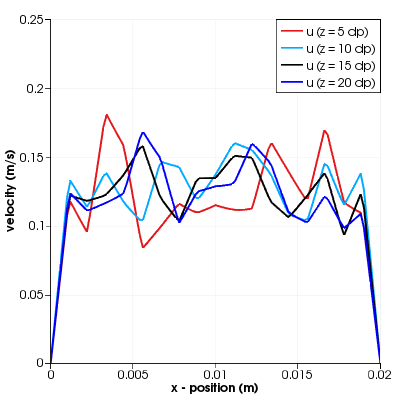
\includegraphics[width=\singleimagewidth]{chapters/figures/lbm/evap-u-profiles}
%     \caption{Velocity profiles (in the $x$-direction) at varying pebble bed heights for the pebble bed with 10\% damaged pebbles.}\label{fig:lbm-evap-u-profile}
% \end{figure}

\begin{figure}[t]
    \centering
    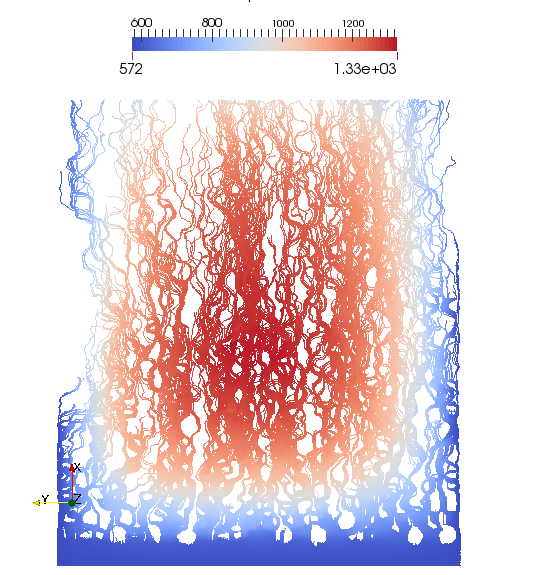
\includegraphics[width=\singleimagewidth]{chapters/figures/lbm/lbm-streamlines}
    \caption{Demonstrating the meandering path -- importantly wandering in the $x$-direction -- of fluid flow in the pebble bed.}\label{fig:lbm-streamlines}
\end{figure}

\begin{figure}[t]
    \centering
    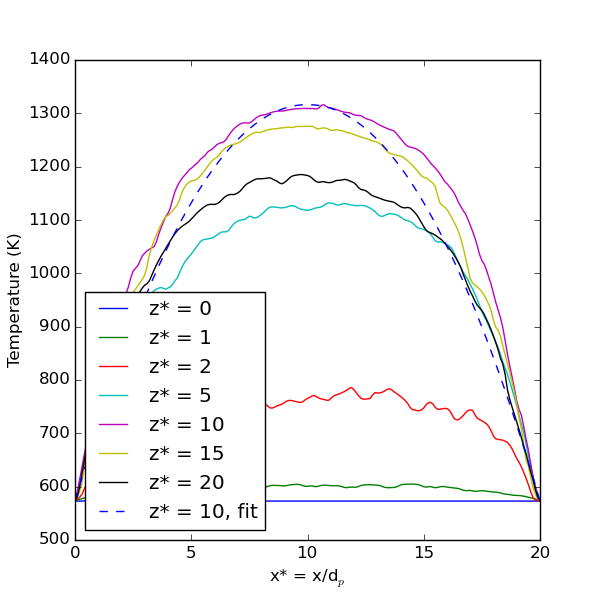
\includegraphics[width=\singleimagewidth]{chapters/figures/lbm/lbm-temp-profiles}
    \caption{Temperature profiles (in the $x$-direction) at varying pebble bed heights for the pebble bed with 10\% damaged pebbles. Shown for comparison is a parabolic profile that had fit both DEM and CFD-DEM temperature results.}\label{fig:lbm-temp-profiles}
\end{figure}

\begin{figure}[t]
    \centering
    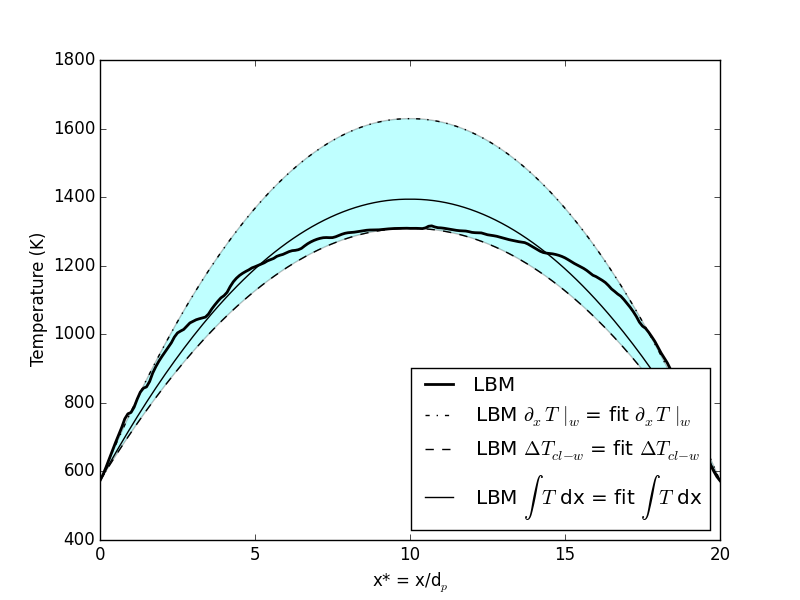
\includegraphics[width=\singleimagewidth]{chapters/figures/lbm/lbm-temp-profile_parabolic}
    \caption{A parabolic fit to the integrated energy of a temperature profile compares to the temperature profile from LBM. The LBM temperature profile increases near the walls and is flattened near the centerline. The behavior is indicative of laminar mixing of energy in the bed.}\label{fig:lbm-temp-parabolas}
\end{figure}

\begin{figure}[t]
    \centering
    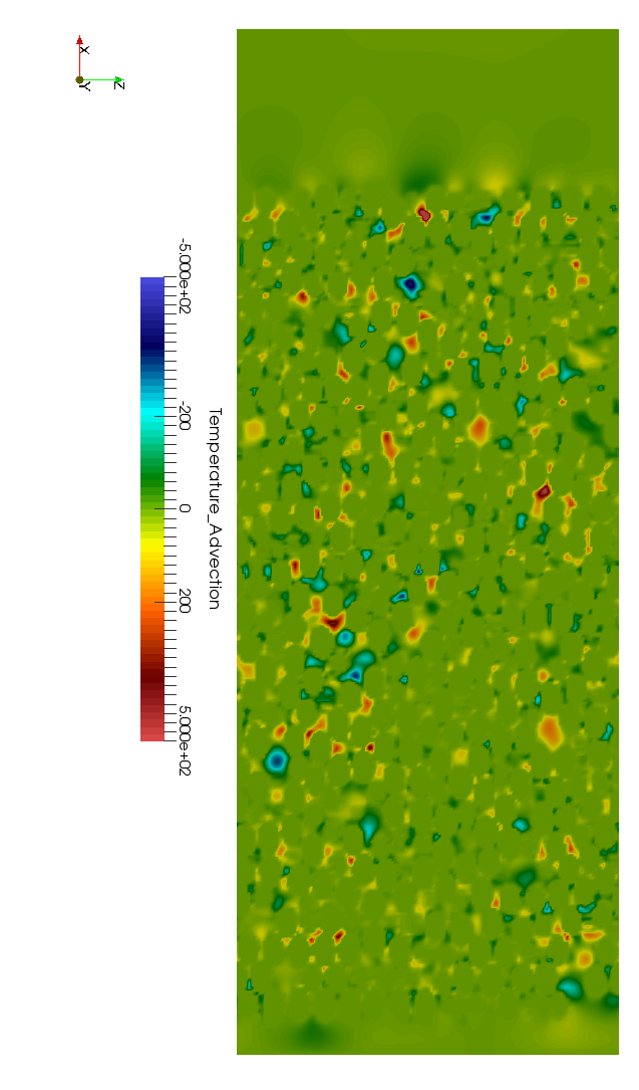
\includegraphics[width=\singleimagewidth]{chapters/figures/lbm/lbm-laminar-mixing}
    \caption{Mean flow direction is in the positive $x$ direction. This $x$-$z$-plane slice shows the $y$ components of velocity as the fluid moves into/out of the plane - mixing the energy with laminar flow.}\label{fig:lbm-laminar-mixing}
\end{figure}

\FloatBarrier